\documentclass[a4j,12pt]{jarticle}
\usepackage{url}
\usepackage{epsfig}
\usepackage{tabularx}
\usepackage{slashbox}
\usepackage{comment}
\usepackage{subfigure}
\usepackage{multirow}

\def\subfigcapskip{0pt}

\usepackage{ccaption}
\setlength{\abovecaptionskip}{0pt}
\setlength{\belowcaptionskip}{0pt}
\setlength\floatsep{20pt}
\setlength\abovecaptionskip{10pt}
\setlength\belowcaptionskip{10pt}

\newlength{\leftcolumn}
\setlength{\leftcolumn}{0.40\textwidth}
\newlength{\rightcolumn}
\setlength{\rightcolumn}{0.55\textwidth}

\addtolength{\topmargin}{-.75cm}
\addtolength{\oddsidemargin}{0.18cm}
\addtolength{\textwidth}{2zw}
\addtolength{\textheight}{0.5cm}
\addtolength{\footskip}{-0.8cm}
\setlength{\parindent}{2.5ex}
\newcommand{\normaldefault}[1]{\default{}{#1}{#1}}
\newcommand{\default}[3]{\frac{#1\,:\,#2}{#3}}

%図が入りやすくなる魔法のコマンド
  \setcounter{topnumber}{9} % 頁上部の最大float数
  \setcounter{totalnumber}{9} % 1頁の 〃
  \setcounter{dbltopnumber}{9} % twocolumn時の頁上部の最大float数
  \renewcommand\topfraction{.9} % 頁上部のfloatで占める最大の割合
  \renewcommand\textfraction{.001} % 1頁のテキスト部の占める最小割合
  \renewcommand\dbltopfraction{.9} % twocolumn時の topfraction
  \renewcommand\dblfloatpagefraction{.9} % twocolumn時の floatpagefraction
%魔法

% \graphicspath{{../image/}}
\begin{document}
\mbox{}
%**まえがき**

%**{表紙}**
%\pagestyle{empty}
%\begin{titlepage}
    \fbox{\Large 2021年1月7日提出}
      \vspace*{160truept}
    \begin{center}
      \fbox{\Large 修士論文}

      \vspace{20truept}
      \fbox{
        \begin{tabular}{c}
          {\Huge エンタテインメントを用いた}\\
          {\Huge プログラミング初学者の}\\
          {\Huge 学習意欲促進システムに関する研究} 
        \end{tabular}
      }

      \vspace{110truept}

      \fbox{
        \begin{tabular}{c}
          {\Large 指導教員:西田健志 准教授}\\
          \vspace{10truept}
          {\Large 副指導教員:大月一弘 教授}
        \end{tabular}
      }
      \vspace{50truept}

      \fbox{
        \begin{tabular}{c}
          {\Large 神戸大学大学院国際文化学研究科}\\
          \vspace{10truept}
          {\Large グローバル文化専攻情報コミュニケーションコース}\\
          \vspace{10truept}
          {\Large 学籍番号・氏名 198c125c 岡 大貴}
        \end{tabular}
      } 

  \end{center}
\end{titlepage}

\pagestyle{myheadings}                       % 右上にページ

\newtheorem{theorem}{定理}       % theorem
\newtheorem{definition}{定義}

\renewcommand{\thepage}{\roman{page}\,\,\,}  % 英語ページ
\setcounter{page}{1}
\setlength{\baselineskip}{21pt}
\begin{center}
  {\Large エンタテインメントを用いた\\プログラミング初学者の\\学習意欲促進システムに関する研究}\\
  \vspace{20truept}
    所属専攻・コース:グローバル文化・情報コミュニケーション\\
    氏名:岡 大貴\\
    指導教員氏名:西田 健志\\
\end{center}

\section*{内容梗概}

プログラミングが重要視されている昨今では,プログラミングの授業が小学校に導入されるなど,プログラミングの一般教養化が推し進められている.しかしプログラミングを楽しむためにはある程度の習熟を必要とし,学習中に挫折してしまうプログラミング初学者も少なくない.プログラミングの楽しさを実感させるための初学者向けプログラミング学習コンテンツも存在するが,その多くは小・中学生を対象として設計されておりそれ以上の年代に対しては効果が薄い場合がある.またビジュアルプログラミング言語を用いているため,実践的なテキストプログラミング言語とは乖離がある場合もある.


そこで本研究では初学者のテキストプログラミング言語を用いた学習・興味喚起を促すため,2つのアプリケーションを開発した.1つ目はエンタテインメントの要素を取り入れることによりコードリーディングを促進するソースコード閲覧システムである.このシステムではクイズ,占いといったエンタテインメントを交えてGitHubにあるソースコードを表示し,ユーザが読解それを読み解くことにより,楽しみながらコードリーディングを促進することを目指した.実装したアプリケーションを使用し運用を行い,その後アンケート調査・ディスカッションを行った結果,クイズに関しては楽しかったという回答が得られたが,ややプログラミング初学者にとっては難解であるという意見が得られた.また表示するソースコードを選択するアルゴリズムの改善や,日常的な使用を促すために更なる工夫が必要であり,これらの問題点を今後改善し,より多くの初学者を対象にワークショップ等を行う予定である.


2つ目はリアルタイム性・アドリブを取り入れた対人形式のプログラミングゲームである.このシステムでは習熟度の高いプログラマ2人がプログラミングスキルによって力量を競って勝負することができ,プログラミング初学者でも観戦して楽しむことができる.このゲームの観戦によってプログラミングへの好奇心を高めるとともに,習熟したプログラマへの憧れを創出することで,初学者のプログラミングに対する興味関心を高めることを目指した.評価実験では実際に2人のプログラマの対戦を初学者に観戦させ,プレイヤであるプログラマと観戦した初学者の双方にアンケート調査を行った.実験結果としてゲームのプレイ・観戦は楽しく,プログラミングに対する興味が高まったなどシステムに対する肯定的な意見が多く得られたが,ゲームシステム・デザインの改善点に関するコメントも多く得られた.またプログラマがプレイ時に記述したプログラムを分析した結果,戦略の多様化・より可読性の高いプログラムの表示などいくつかの改善点が見つかった.

この結果を受け,今後は提案システムを改善すると共に,より多くのプログラミング初学者を含むプログラマにシステムを使用させ,より良いシステムの構築を目指す.

\newpage
\markright{}
\tableofcontents            %  目次
\markright{}
\newpage

%###################### 本文 #######################
\renewcommand{\thepage}{\arabic{page}\,\,\,}  % 数字ページ

\setcounter{page}{1}
\setlength{\baselineskip}{19pt}

\newpage
\section{はじめに}

高速にIT化の進む近年では,IoT,AI,クラウドコンピューティングといった単語がメディアで散見されるようになり,誰もがスマートフォンを持ち,TwitterやYouTubeなどのソフトウェアを利用するようになった.家電や自動車,学校教育にもコンピュータが導入され,コンピュータが着実に人々の生活を満たしつつあるといえる.コンピュータが遍在する現代において,人とコンピュータの接点は圧倒的に多くなり,コンピュータを専門的に扱う人でなくともそれに触れて暮らすことが当たり前となっている.就労などの社会活動においても,あるソフトウェアを使いこなせたり,プログラミングができるなどコンピュータとの親和性が高いことがアドバンテージとなる場合もある.

近年ではその高速な社会のIT化に伴い,プログラミングが重要性を増している.国際的には,ロシアでは2009年からプログラミング教育が導入され,英国では2014年から「Computing」というコンピュータサイエンス,情報技術,デジタルリテラシーの3分野からなる科目が導入されており\cite{survey},日本においても今年度から小学校でのプログラミング教育が必修化されている\cite{guide}.以前は「プログラミングはエンジニアや理系の学生がやるもの」というような,専門家だけの技能であるという認識が強かったが,プログラミングが英語のように一般教養となり,プログラミングに関わる仕事に就かない人もある程度理解していることが求められている.

% プログラミングという行為はコンピュータを活用し,ソフトウェア開発・ハードウェア制御などにより人々の活動の生産性を高めるだけでなく,自身のアイディアをコンピュータを介して表現する手段でもあり,プログラミングスキルを向上させることは自己表現の可能性を広げることにつながる.近年ではProcessingやopenFrameworks,Arduinoなどの登場により,プログラミングにより創造的な表現を生み出す「クリエイティブ・コーディング」やメイカームーブメントが流行し,コンピュータ・サイエンス等の知識がなくともプログラミングによってものづくりをし,発表できる土壌が整いつつある.

しかしプログラミング教育の現場やその学習教材では,プログラミングの機能にのみ焦点が当たりがちで,プログラミングの「楽しさ」が疎かにされていることが少なくない.プログラミングをする上で楽しさを感じることは,学習の観点からも重要である.松本らによるC言語プログラミングの授業では、学習の楽しさや、プログラミングへの興味が高いほど授業の学習率が高いことが示されている\cite{matsumoto}.

しかし最初から理解が容易で楽しさを感じやすい読み書きや運動とは異なり,プログラミングは楽しさを感じるまでにある程度の習熟を要する.よく書かれた小説などの文章やプロスポーツでのファインプレーには初心者でも心動かされるもので,そうした小説家やスポーツ選手への憧れが自ら書くことや体を動かすへの感心を高めるが,プログラミングの場合にはそのような憧れをもつ機会に乏しいのが現状である.

プログラミング初学者にプログラミングの楽しさを実感させるために設計された学習コンテンツは多数存在し,ScratchやViscuitなどのビジュアルプログラミング言語(VPL: Visual Programming Language)がその代表的な例である.これらは実際に学校教育で導入され,小・中学生のプログラミング教育に貢献している.しかしそれらは小・中学生など若い年代をターゲットに設計されているため,高校生や大学生,それ以上の年代にとっては楽しさを感じにくい場合がある.また実践的なソフトウェア開発においてはテキストプログラミング言語(TPL: Textual Programming Language)を用いる場合がほとんどであるため,VPLとTPLの間に乖離があることも問題である.

本研究では従来のシステムがターゲットとしている世代よりも上の世代のプログラミング初学者を対象に,エンタテインメントの要素を用いることでプログラミングに対する抵抗感を減らし,プログラムを書かずともプログラミングを楽しんでもらうためのシステムの開発を目指した.具体的には初学者のコードリーディングを促進するアプリケーション,プログラミングゲームを用いてプログラミングに対する興味喚起を行うアプリケーションの2つを開発し,それぞれ初学者を対象に運用を行うことでその効果を検証した.


本論文では以降,2章で研究指針について述べた後,3章でゲーミフィケーションを用いたコードリーディング促進システムについて述べ,4章でプログラミング初学者の興味喚起を目的としたプログラミングゲームについて述べる.5章で本論文をまとめる.
\markright{}

\newpage
\section{コードリーディング支援システムに関する研究}

プログラミングの重要性の高まりに伴い,プログラミングを学ぼうとする人が増えている.そういった人には書籍や学習用webサイトを通して学ぶ場合と情報系の学校やプログラミングスクールなどに通ってプログラミングスキルを身につけようとするパタンがあるが,学習にかかる費用や時間が取れないなどの理由から前者を選ぶ人が多い.

初学者向けプログラミング学習コンテンツが普及し,プログラミング入門のハードルは下がってきているものの,それらではプログラムを「書く」ことに千年させるものが多い.例えばプログラミング学習サイトであるProgate\cite{progate}では,主要なプログラミング言語の文法やライブラリの用法など,「どうプログラムを書くか」を重点的に教えている.

しかしプログラミング学習において重要とされているスキルは様々である.プログラムを書くスキルだけでなく,論理的思考力,コードリーディングスキル,情報収集スキルなど多くの技術を必要とし,これらを網羅的に学習教材を通して身につけるのは難しい.

本項で提案するシステムでは,その中でもコードリーディングスキルに焦点を当て,エンタテインメントの要素を組み込んでプログラムを閲覧させることにより,プログラミング初学者のコードリーディングを促進するシステムを開発した.
\subsection{関連研究}

GitHubを活用した研究はいくつかある.永野らの研究\cite{nagano}ではGitHubとStackOverflowのデータを用いて双方を利用するユーザについて調査している.この研究ではユーザがGitHubで作成したリポジトリとStackOverflowへの投稿のコンテンツの関連性について調べたもので,双方への投稿コンテンツに一定の相関があることを示している.また柴藤らはGitHub上の断片データに関する情報を取得できるシステムを開発している\cite{shibatou}.このシステムではユーザが指定したソースコード中の一部の連続したコードに関するプルリクエストを取得できるというものであり,ソースコードを閲覧する際の利便性を高めている.

またエンタテインメントの要素,特にゲーミフィケーションを活用した研究も盛んである.一ノ瀬らの研究\cite{ichinose}ではソースコード上の技術的負債を可視化し,さらにゲーミフィケーションの要素を加えることで技術的負債の除去を促している.この研究ではソースコードのファイル構造を街のように可視化し,技術的負債が存在するファイルを目立たせ,さらに技術的負債を取り除いたユーザをランキング形式で表示することによって,ゲーミフィケーションの要素を元に生産的な行動を促している.

なおコードリーディング支援に関してもいくつか研究がなされており,大村らや石尾らはソースコードを読解する際のコードリーディング支援を行うツールを開発している\cite{omura}\cite{ishio}.
しかし,これらの研究ではある程度プログラミングに習熟したプログラマがソースコードを読むという状況を想定しているため,コードに触れる機会を増やすための本研究とは目的が異なる.

\subsection{設計指針}
システムを実装するにあたり以下の設計指針を設けた.
\begin{enumerate}
  \item 遊び(エンタテインメント)の要素を取り入れる

  コードリーディングはプログラミングにおいて重要なスキルの1つであるが,プログラムを読解する経験の少ないプログラミング初学者にとって,淡白なプログラムをただ読み込むことは難しい.よってエンタテインメントの要素を付与してプログラムを読ませることで,コードリーディングの心理的障壁を下げることを目指した.
  \item 日常的に使用するツールに組み込む

  アスリートが継続的なトレーニングを怠らないように,ある技能を高めるには日常的な鍛錬を要する.プログラミングにおけるコードリーディングでも同様であると考え,極力システム利用のハードルを下げるためにシステムを日常的に使用するデバイス・アプリケーションから使用できるように設計した.
  \item プログラムを読むことに専念させる

  プログラムの記述を促進するならば対象のソースコードを1つの言語に絞るべきという考え方もある.コードを書くことが目的であれば,複数の言語を同時進行させることは混乱を招き,デメリットが大きい.しかし,コードを読むことが目的であれば,上級者との会話のきっかけができる,将来的に適材適所で言語を使い分けることにつながる,飽きずにシステムを使用させ,コードの読解に興味を持たせることにつながるなどメリットが大きい,従って本システムでは,多様な言語に触れられる機能と1つの言語に読解を絞った機能を実装した.
\end{enumerate}

\subsection{提案システム}
\subsubsection{実装機能}
システムで使用できる2つの機能について説明する.
\begin{enumerate}
  \item クイズ機能

  この機能はユーザが使用した際にGitHubから取得したランダムなプログラムを表示する.ユーザは表示されたプログラムを読み,どのプログラミング言語で記述されたプログラムかを回答する.正解した場合は得点が得られ,取得した累計得点の多さによるランキングが表示される.

  \item 占い機能

  この機能をユーザが使用するとGitHubからランダムに得られたプログラムが表示され,ユーザはそれを読解し自分なりの解釈をすることで,その日の運勢を占う.表示されたソースコードの意味を解釈することが必要であるため,必然的にコードの読解が必要となる.この機能においては表示されるプログラムをJavaScriptで記述されたもののみにした.

\end{enumerate}
\subsection{プロトタイプシステム}
初めに,提案システムをチームコミュニケーションツールであるSlackのbotとして実装した.システムを利用する際は,このbotを導入しているチャンネルでコマンドを入力することで各機能を使用できる.利用可能なコマンドを表\ref{function}に示す.またクイズ機能の様子を図\ref{prototype_quiz}に,占い機能の様子を図\ref{prototype_fortune}に示す.

\begin{figure}[!ht]
  \begin{center}
    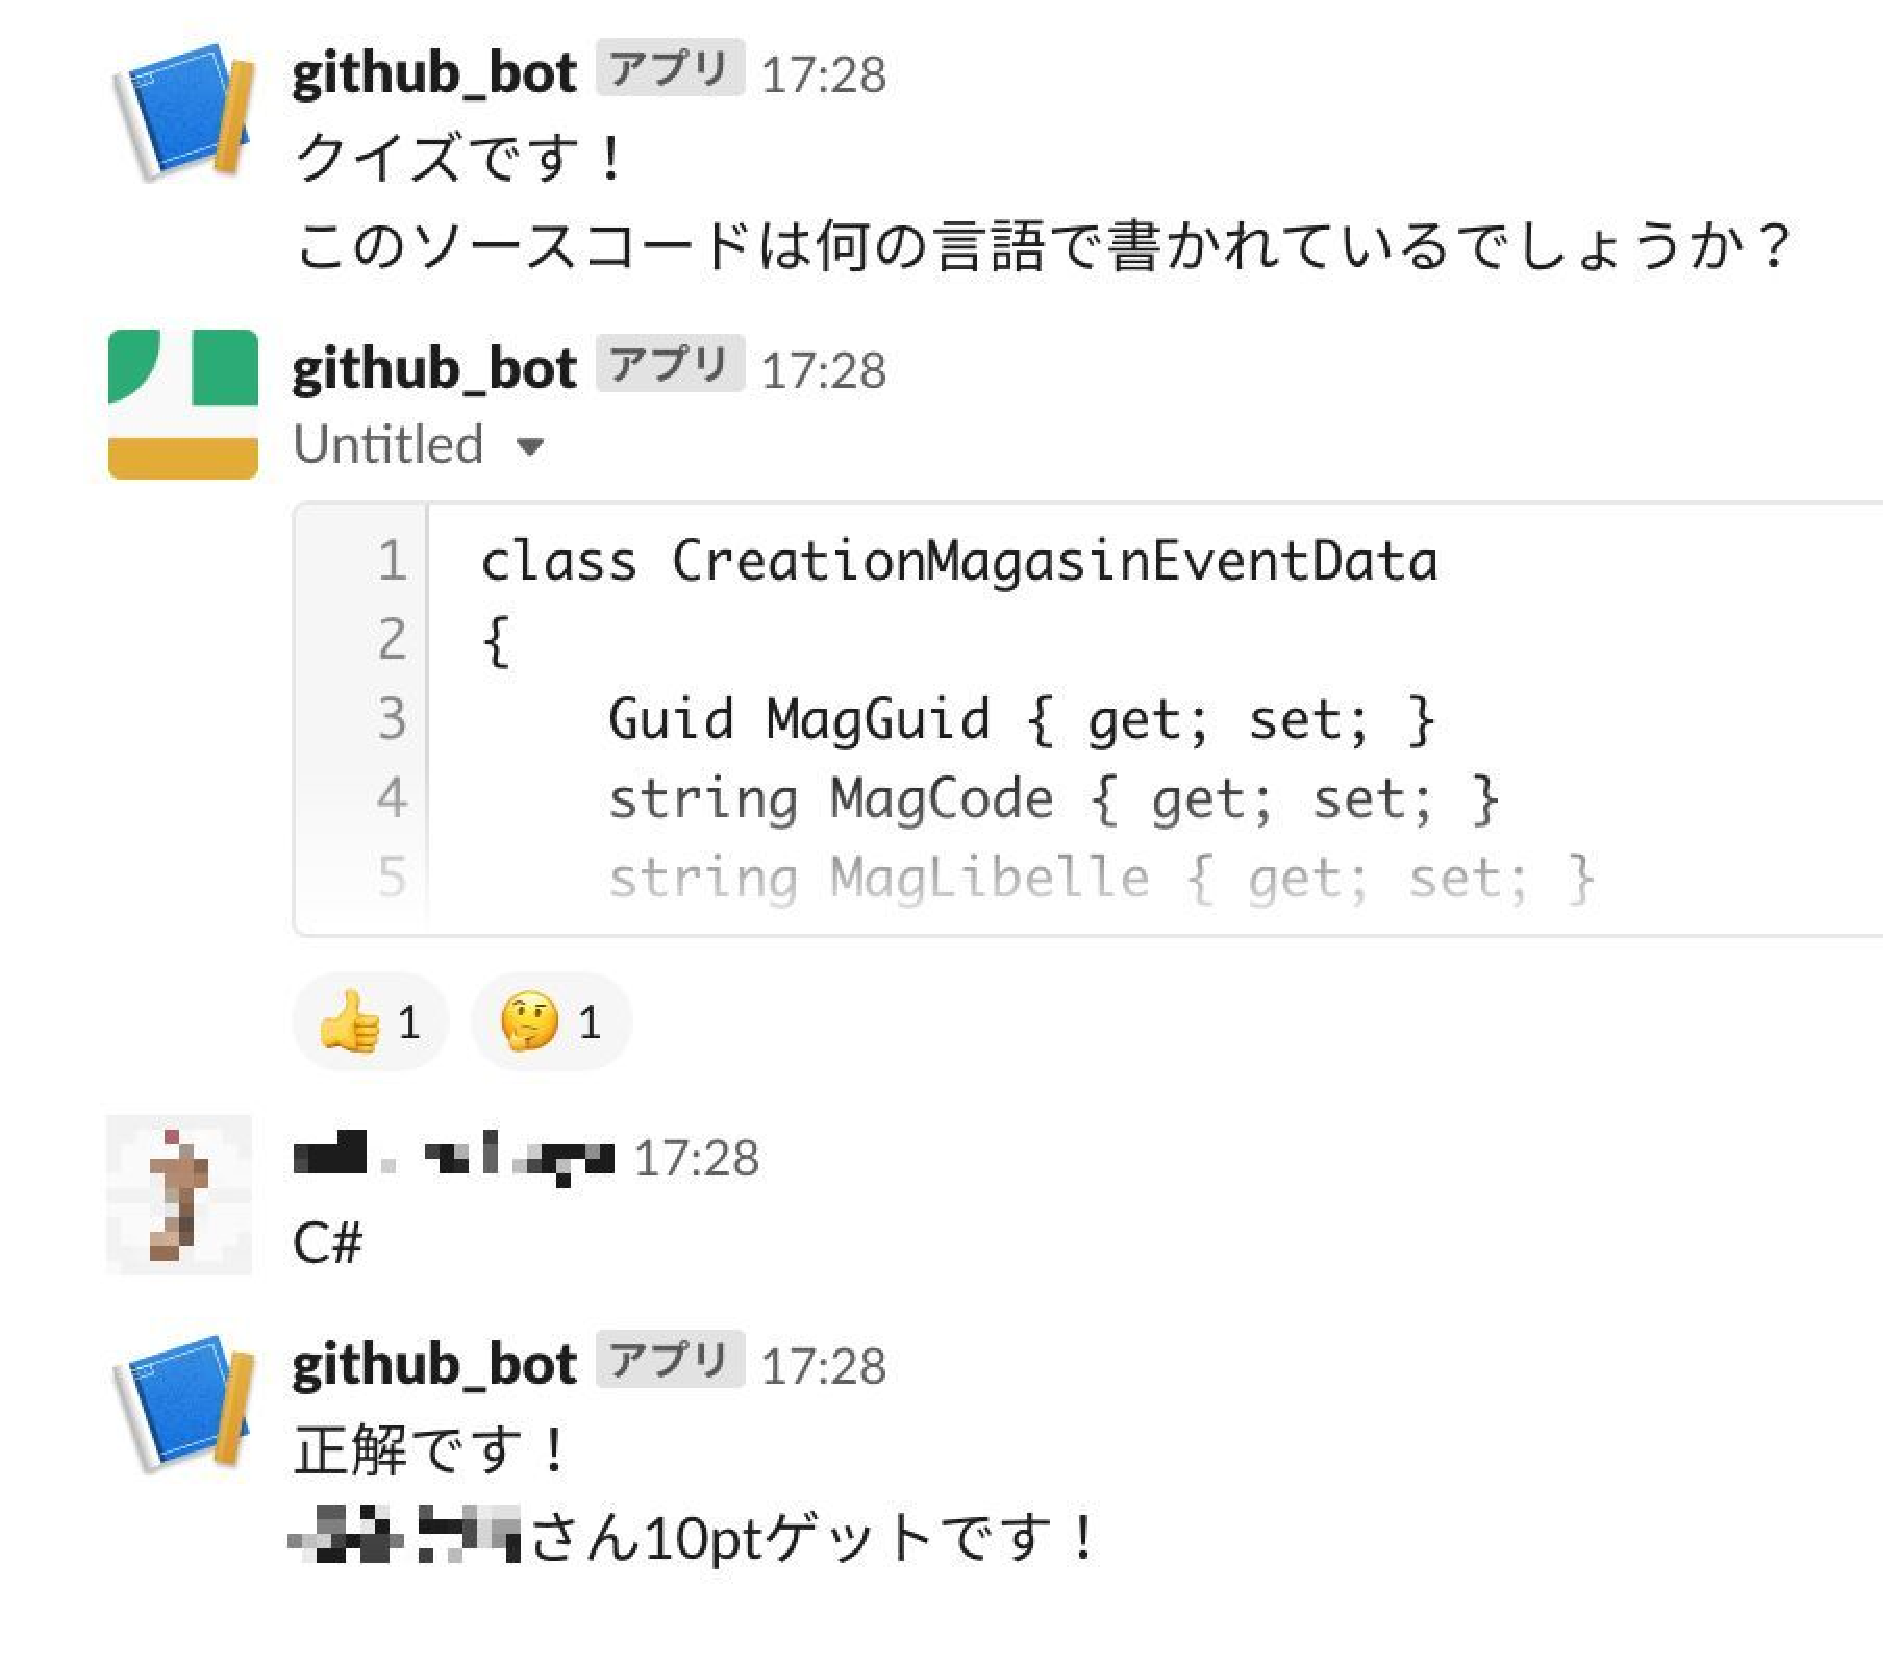
\includegraphics[width=0.6\linewidth]{image/prototype_quiz.eps}
  \end{center}
    % \vspace{-8mm} 
  \caption{クイズ機能の様子}
  \label{prototype_quiz}
\end{figure}

\begin{figure}[!ht]
  \begin{center}
    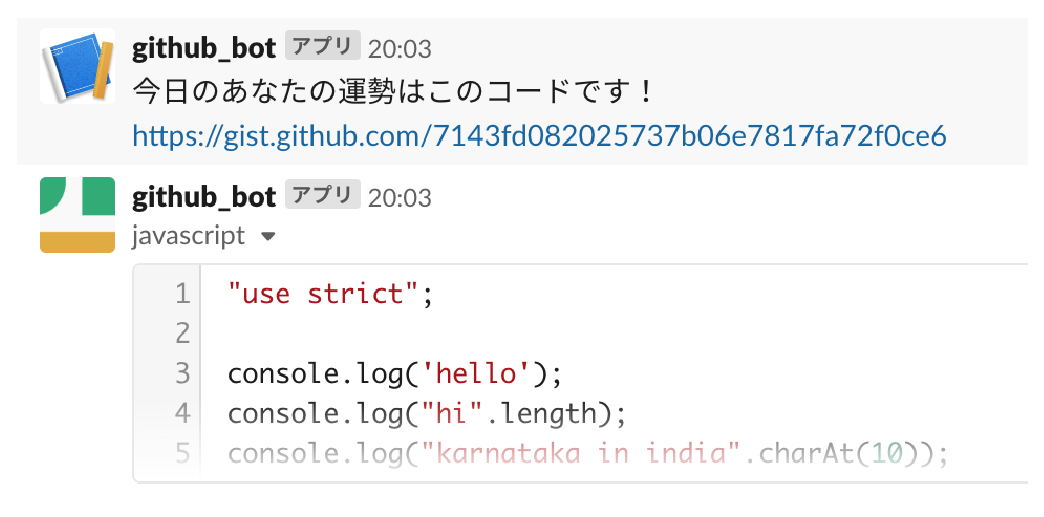
\includegraphics[width=0.6\linewidth]{image/prototype_fortune.eps}
  \end{center}
    \vspace{-8mm} 
  \caption{占い機能の様子}
  \label{prototype_fortune}
\end{figure}

\begin{table}[!ht]
  \centering
    \caption{コマンド一覧}
      \begin{tabular}{|c|c|} \hline
        コマンド & 説明 \\ \hline \hline
        fortune & 1日の運勢を占うソースコードを表示 \\ \hline
        quiz & 記述言語を問うクイズを出題 \\ \hline
        hint & クイズに関するヒントを表示 \\ \hline
        answer & クイズの回答を表示 \\ \hline
        score & 各ユーザの累計得点を表示 \\ \hline
      \end{tabular}
    \label{function}
  \end{table}

\subsubsection{ケーススタディ}
このシステムを筆者が所属する研究室のSlackに導入し,研究室のメンバーを対象としたケーススタディを行った..研究室のメンバーは3名のプログラミング初学者であり,1週間自由に機能を使用してもらい,各コマンドの使用回数を調べた.またアンケートによって所感を調査した.アンケートの内容を以下に示す.

\begin{itemize}
  \item どういう状況で機能を使用したか
  \item 占い機能について,楽しかったか(5段階評価,1:楽しくなかった,5:楽しかった)
  \item 占い機能について,どういう点が楽しかった(楽しくなかった)か
  \item クイズ機能について,楽しかったか(5段階評価,1:楽しくなかった,5:楽しかった)
  \item クイズ機能について,どういう点が楽しかった(楽しくなかった)か
  \item 機能を使用したことによって学びがあったか
  \item どういう学びがあったか
  \item コードを読むことへの抵抗は減ったと感じるか(5段階評価,1:減らなかった,5:減った)
  \item 今後も機能を使いたいか
  \item 感想,意見,改善点など
\end{itemize}

各コマンドの使用回数を表\ref{command}に示す.

\begin{table}[!ht]
  \centering
  \caption{各コマンドの使用回数}
  \label{command}
    \begin{tabular}{|c|c|} \hline
      コマンド & 使用回数 \\ \hline \hline
      fortune & 9 \\ \hline
      quiz & 43 \\ \hline
      hint & 27 \\ \hline
      answer & 3 \\ \hline
      score & 33 \\ \hline
    \end{tabular}
\end{table}

コマンドの使用回数に関しては,クイズ機能に関連した機能が多い結果となり,占い機能に関しては使用回数が少なかった.また期間中の最初の3日間ほどは頻繁にシステムが使用されていたが,期間の後半おいてはあまり活発に使用されていなかった.またどの機能も個別に使用するより,ユーザが実際に会って集まっている際にコミュニケーションを交えて使用されることが多かった.

次にアンケート結果を表\ref{interview}に示す.
\begin{table}[!ht]
  \centering
  \caption{アンケート結果}
  \label{interview}
    \begin{tabular}{|c|c|c|c|} \hline
      インタビュー内容 & 被験者A & 被験者B & 被験者C \\ \hline \hline
      占い機能は楽しかったか & 1 & 2 & 3 \\ \hline
      クイズ機能は楽しかったか & 4 & 4 & 5 \\ \hline
      コードへの抵抗感は減ったか & 3 & 5 &5 \\ \hline
    \end{tabular}
\end{table}

まず占い機能に関してだが,使用する楽しさの評価は低い結果となった.ユーザの意見には「提示されたプログラムをどう解釈すればいいのか分からなかった」「占いという感触があまりなかった」などがあり,プログラミング初学者にとってプログラムを読解して独自の解釈を持たせることは難しく,面白みに欠けているようだった.
またクイズ機能に関しては楽しさに関して高い評価が得られた.その理由として「スコアがあると、競争している感が出るところが楽しく感じた」「みんなで一緒にやっていて競争っぽくなるとき楽しかった」などの意見があり,スコアを用いたゲーミフィケーション,競争の要素がシステム使用のモチベーションを高めていた.また「以前に出た言語の特徴に似ていると感じ、調べずに答えて正解したとき楽しかった」という意見が得られ,クイズを通したコードリーディングによってプログラミング言語の特徴を捉え,それに楽しみを感じていることが分かった.
なお「機能を使用したことによって学びがあったか」という質問には全員が「あった」と回答し,「どういう学びがあったか」という質問には「言語ごとの文法の特徴が何となく分かってきた」「いろんな言語の存在を知ることができました」「今まで聞いたこともなかったプログラミング言語の名前を知り、親近感をもった」という回答があり,各プログラミング言語の特徴について理解するとともにプログラミングに対する親近感を抱かせることができていた.またコードへの抵抗感に関する質問でも肯定的な評価が得られ,「今後も機能を使いたいか」という質問に対して全員が「使いたい」と回答した.なおシステムの改善点に関して「プログラムのあるGitHubのページへのリンクを表示して欲しい」「占いの際にラッキーアイテムなどを表示して欲しい」等の意見が得られたため,アンケート結果を元にプロトタイプを改善したシステムを開発した.

\subsection{Webアプリケーション}
プロトタイプシステムを用いたケーススタディで得られた結果を元に,プロトタイプシステムを改善し,Webアプリケーションとして再実装した.Webアプリケーションとして実装したのはSlack botよりも開けたコミュニティでより多くのユーザの意見を取り入れるためである.このアプリケーションでは指定のURLにアクセスすることでクイズ・占いの機能を使用でき,ユーザ登録をしログインすることでクイズ正解時に得た得点の累計によるユーザのランキングを閲覧することができる.またクイズ機能においてはそのクイズに対するユーザの正答率,占い機能においては選ばれたプログラムに含まれているコメントの量,宣言された関数の数などから独自に算出した対人運,仕事運,コメントなどを表示するようにした.クイズ機能の様子を\ref{quiz}に,占い機能の様子を\ref{fortune}に示す.
また実装したアプリケーションをUbiquitous Wearable Workshop2019にて参加者に使用させた.占い・クイズ機能ともに使用され,表示されたプログラムを見せ合うなどシステムを介したコミュニケーションが見られたが,「クイズが難しすぎて逆にプログラムに対する抵抗感が生まれた」というコメントもあった.

\begin{figure}[!ht]
  \begin{center}
    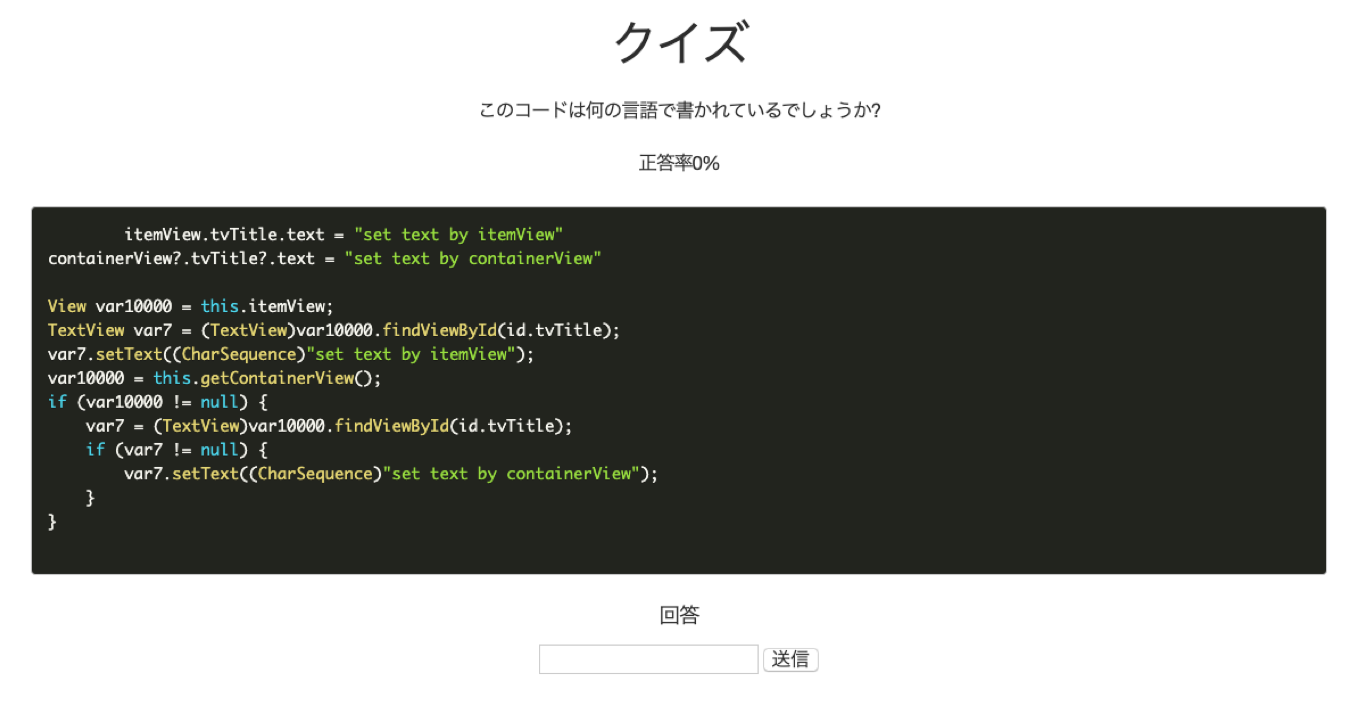
\includegraphics[width=1.0\linewidth]{image/quiz.eps}
  \end{center}
    \vspace{-8mm} 
  \caption{クイズ機能の様子}
  \label{quiz}
\end{figure}

\begin{figure}[!ht]
  \begin{center}
    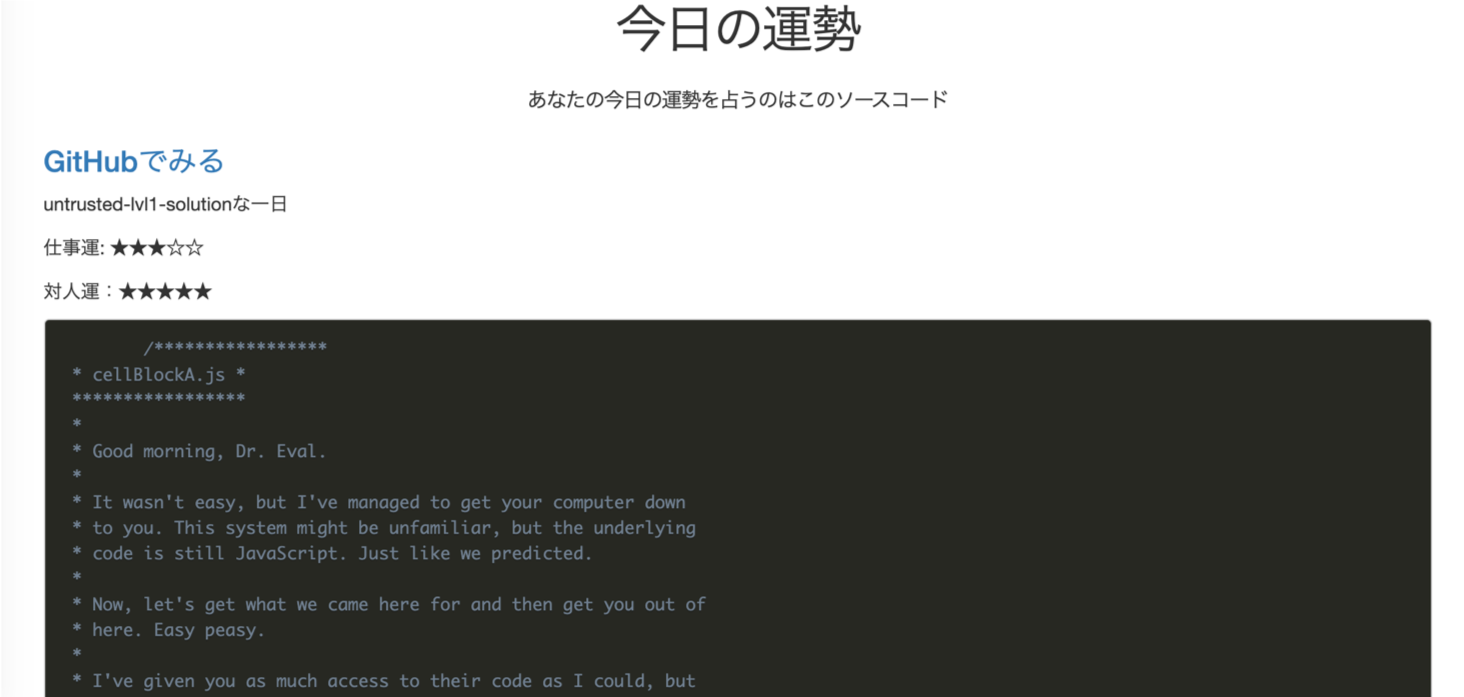
\includegraphics[width=1.0\linewidth]{image/fortune.eps}
  \end{center}
    \vspace{-8mm} 
  \caption{占い機能の様子}
  \label{fortune}
\end{figure}


\subsection{課題と考察}
提案システムの実装と運用を通して,エンタテインメントの要素,特にクイズの要素を交えてプログラミング初学者のコードリーディングを促進することは,有効な方策であると考えられる.またその中で他者と競争するゲーミフィケーションはシステム使用のモチベーションとなり,これをプログラミング学習に取り込むことで有益な学習コンテンツを作成できると感じた.しかし,現状実装したアプリケーションには不十分な箇所が多く,より適切なゲームデザイン,ユーザがシステムを使い続けるための工夫,どのようなアルゴリズムでプログラムを選び,初学者に提示するかなど課題は多い.今後はこのシステムを通して得られた課題・観点を元に,より良いプログラミング学習コンテンツを作成していく.


\newpage
\section{競技性・観戦性を拡張したプログラミングゲームの開発}
本項では,プログラミング初学者の興味喚起を目的としたプログラミングゲームのプロトタイプについて紹介し,設計指針に基づくデザインの詳細や行った評価実験と見つかった課題,実験に関する考察について議論する.

\subsection{関連研究・関連システム}

\subsubsection{プログラミングを用いたエンタテインメントシステム}
プログラミングとエンタテインメントを掛け合わせたコンテンツはいくつか存在する.TopCoder\cite{topcoder}などの競技プログラミングやコードゴルフ\cite{codegolf},SECCON\cite{seccon}などのハッキングコンテストが有名であり,プログラマの間でも根強い人気がある.またプログラミングゲームとしてはRobocode\cite{robocode}が有名である.しかしこれらはある程度プログラミングに習熟したプログラマ向けのコンテンツであるため,数学やセキュリティ,コンピュータサイエンス等の知識を要するためプログラミング初学者が参加するにはハードルが高い.

\subsubsection{初学者向けプログラミング学習支援システム}
初学者向けプログラミング学習支援システムは数多く存在する.Scratch\cite{scratch},Viscuit\cite{viscuit}などはその代表的な例であり,低年齢層をターゲットにした設計でブロックや絵を並べることでプログラミングでき,初学者にプログラミングの楽しさを伝えるためにデザインされている.またドリトル\cite{dolittle}は中学校・高等学校での教育目的に使える環境を目指し,テキストベースでプログラミングさせつつも柔軟かつ小さい言語仕様により,初学者にプログラミングの楽しさを伝えることを目指している.しかしプログラマに対する憧れを創出し,プログラミングへのモチベーションを高めるという本研究のアプローチとは異なる.

\subsubsection{エンタテインメントを活用したプログラミング学習支援システム}
エンタテインメントの要素を盛り込むことでプログラミング学習を促進しようとした研究は多くある.Joshaらはプログラミングゲームを用いてプログラミング初学者の問題解決能力を向上させるためのシステムを作成している\cite{joshua}.また水口の研究ではプログラミングの講義における成績評価にロボットバトルシミュレーション型のプログラミングゲームを活用している\cite{minakuchi}.三谷らの研究ではキャラクタをプログラムで制御するプログラミングゲームでプログラミングスキルの向上を図っている\cite{mitani}.なお増谷らの開発したVLogic\cite{mashitani}ではVR空間上にブロックベースのプログラミングゲームを実装することで手足を使ってプログラミングを体験することができ,プログラミングに対する興味喚起を行っている.これらはプログラミングの習熟度が高くなくても使用できるが,従来のプログラミングゲーム同様静的なゲーム展開であり,プログラマ同士のリアルタイムな駆け引きやアドリブといった観戦を楽しむ設計は成されていない.



\subsection{設計指針}

提案システムの実装にあたり,初学者の興味関心を高めるために3つの設計指針を設けた.

\begin{enumerate}
	\item 観戦するにあたり,高度な専門知識を必要としない
	
	初学者が提案システムでの対戦を観戦するにあたり高度な専門知識を必要としてしまっては,利用の心理的ハードルを上げかねない.極力前提知識なしに理解し,楽しめるようにデザインする必要がある.
	
	\item 手間がかからない

	初学者にとってプログラミング学習をする際に環境構築や普段使用しない独自ソフトウェアのインストールはモチベーションを下げかねない.今回は提案システムをJavaScriptによって制御可能なWebアプリケーションとして実装し,初学者が実際にプログラミングを行わずとも見るだけで利用できるようにした.
	
	\item リアルタイムな駆け引き・アドリブを取り入れる

	従来のプログラミング教育コンテンツとは異なり,スポーツなどの観戦する競技で見られるようなリアルタイムな駆け引き・アドリブの要素を提案システムに組み込むことで観戦して楽しめるようなデザインをする.
\end{enumerate}

\subsection{提案システム}

本研究で提案するシステムでは,プログラミング初学者の興味喚起をするためにいくつかの工夫を施した.今回実装したシステムは,プログラマ同士がリアルタイムにプログラミングを行うことでキャラクタを制御し,対戦するという対人形式のプログラミングゲームである.この対戦の様子を初学者に観戦させることで,初学者のプログラミングに対する興味を高める.プログラミングゲームとして実装した理由としては,キャラクタがプログラムによって動作するというゲームの視覚的な出力が,初学者にとってプログラムの出力を理解する助けになると考えたためである.ゲームジャンルとしては,シューティングゲームの体裁をとった.これはシューティングゲームが「敵の攻撃を避けて,敵を攻撃する」というプリミティブなゲームシステムであり,見ていて展開を理解しやすいと考えたためである.またゲームUIはLivecodeLabやHydraなどのビジュアルライブコーディング環境を踏襲し,ゲーム画面上にエディタを重畳することで,プログラムとその出力の双方を同時に見ることが可能なように設計した.またゲームは以下の3つのフェイズに分かれている.

\subsubsection{自機プログラミングフェイズ}
対戦が開始するとこのフェイズに移行する.ここでは予めエディタにプレイヤが操作するキャラクタのコンストラクタが記述されており,プレイヤはパラメータを書き換えることができる.具体的なパラメータにはappearance,life,clock,powerがある.appearanceはキャラクタの外見であり,文字列を指定できるため,絵文字などを使ってプレイヤの好きな見た目を選ぶことが可能である.lifeはキャラクタの体力であり,いわゆるHP(ヒットポイント)を表している.非負の整数を指定でき,この値が0以下になるとプレイヤはゲームに敗北する.clockはキャラクタが行動できる回数の多さを表しており,非負の整数を指定できる.プレイヤは後述する行動プログラミングフェイズにおいて自分のキャラクタを制御するプログラムを記述し対戦するが,その際に記述したプログラムは10秒間ループして実行される.このループのインターバルを決めるのがclockであり,値が大きいほどインターバルは短くなる.powerはキャラクタの攻撃力を表しており,これも非負の整数を指定できる.この値が大きいほど,自分が操作するキャラクタの攻撃が相手キャラクタに命中した際に削るlifeの値が大きくなる.双方のプレイヤが各パラメータを記述し終わると次の行動プログラミングフェイズに移行する.このフェイズの様子を図\ref{characterProgramming}に示す.

\begin{figure}[!h]
  \begin{center}
    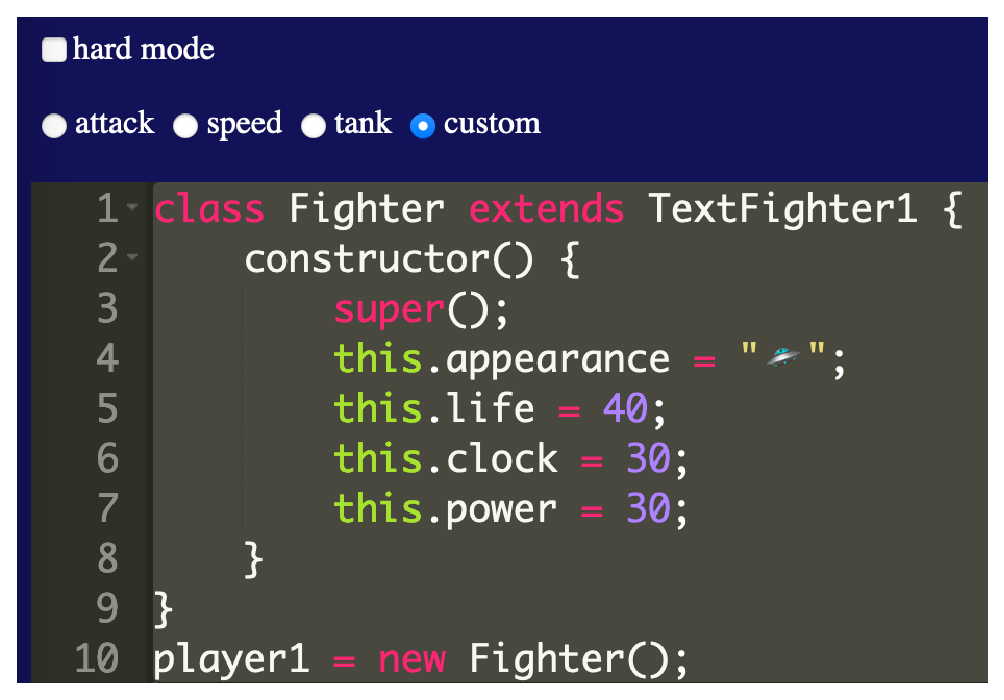
\includegraphics[width=1.0\linewidth]{image/characterProgramming.eps}
  \end{center}
    \vspace{-8mm} 
  \caption{自機プログラミングフェイズの様子}
  \label{characterProgramming}
\end{figure}

\subsubsection{行動プログラミングフェイズ}
このフェイズに進むと,自機プログラミングフェイズで記述したコンストラクタを元に各プレイヤが操作するキャラクタのインスタンスが作成され,ゲーム画面が表示される.各プレイヤはプログラムをエディタに記述し,作成したキャラクタを操作する.プレイヤは条件分岐や繰り返しなど従来のJavaScriptの文法の他に独自に用意されたプロトタイプメソッドを使うことができる.用意したメソッドにはキャラクタを移動するメソッド(moveUp(), moveDown(),randomMove())とキャラクタが攻撃を行うメソッド(shot())などがある.またプログラム内で各キャラクタのパラメータを参照することもできる.両プレイヤがプログラムを記述し終わると次のゲームフェイズに移行する.なおこのフェイズでは相手プレイヤがどのようなプログラムを記述しているかは見ることができない.このフェイズの様子を図\ref{actionProgramming}に示す.

\begin{figure}[!h]
  \begin{center}
    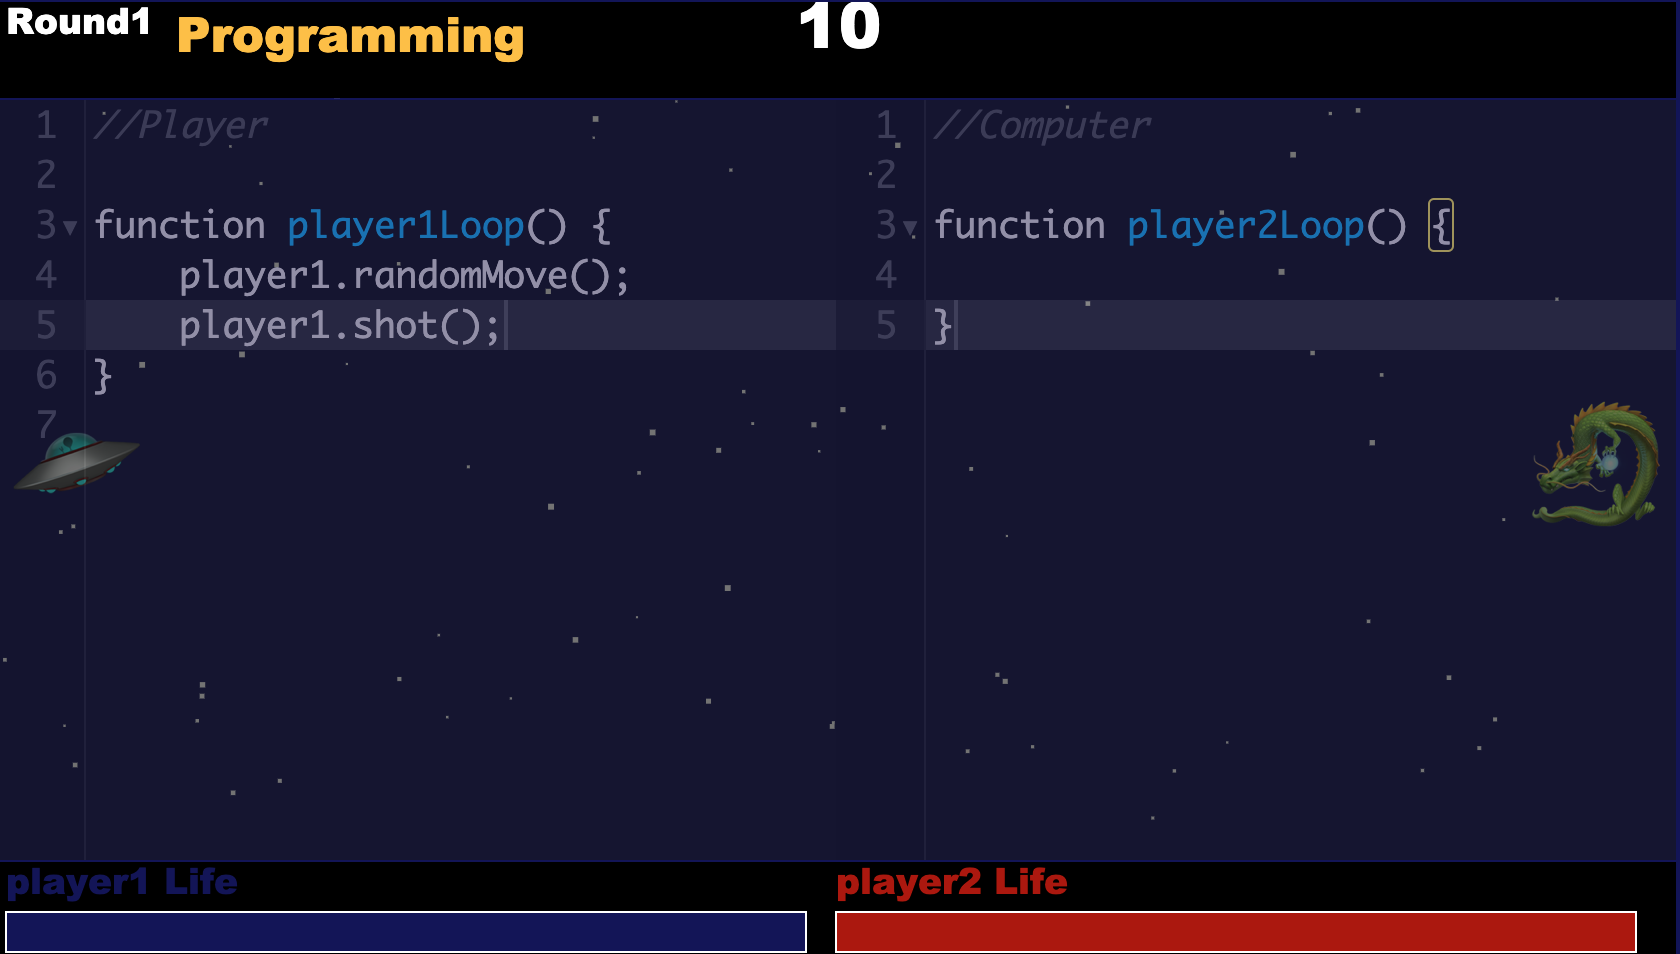
\includegraphics[width=1.0\linewidth]{image/actionProgramming.eps}
  \end{center}
    \vspace{-8mm} 
  \caption{行動プログラミングフェイズの様子}
  \label{actionProgramming}
\end{figure}

\subsubsection{ゲームフェイズ}
このフェイズでは行動プログラミングフェイズで記述したプログラムが10秒間ループして実行され,ゲームが進行する.この段階で両プレイヤは相手プレイヤが記述したプログラムを閲覧することができる.このフェイズにおいて相手キャラクタを攻撃し,lifeの値を0いかにしたプレイヤの勝利となる.勝敗が決まらない場合はプログラム終了時の各パラメータを引き継いだまま行動プログラミングフェイズに戻り,再度プログラミングしゲームフェイズに移行するという過程を勝敗が決まるまで繰り返す.このフェイズの様子を図\ref{game}に示す.

\begin{figure}[!h]
  \begin{center}
    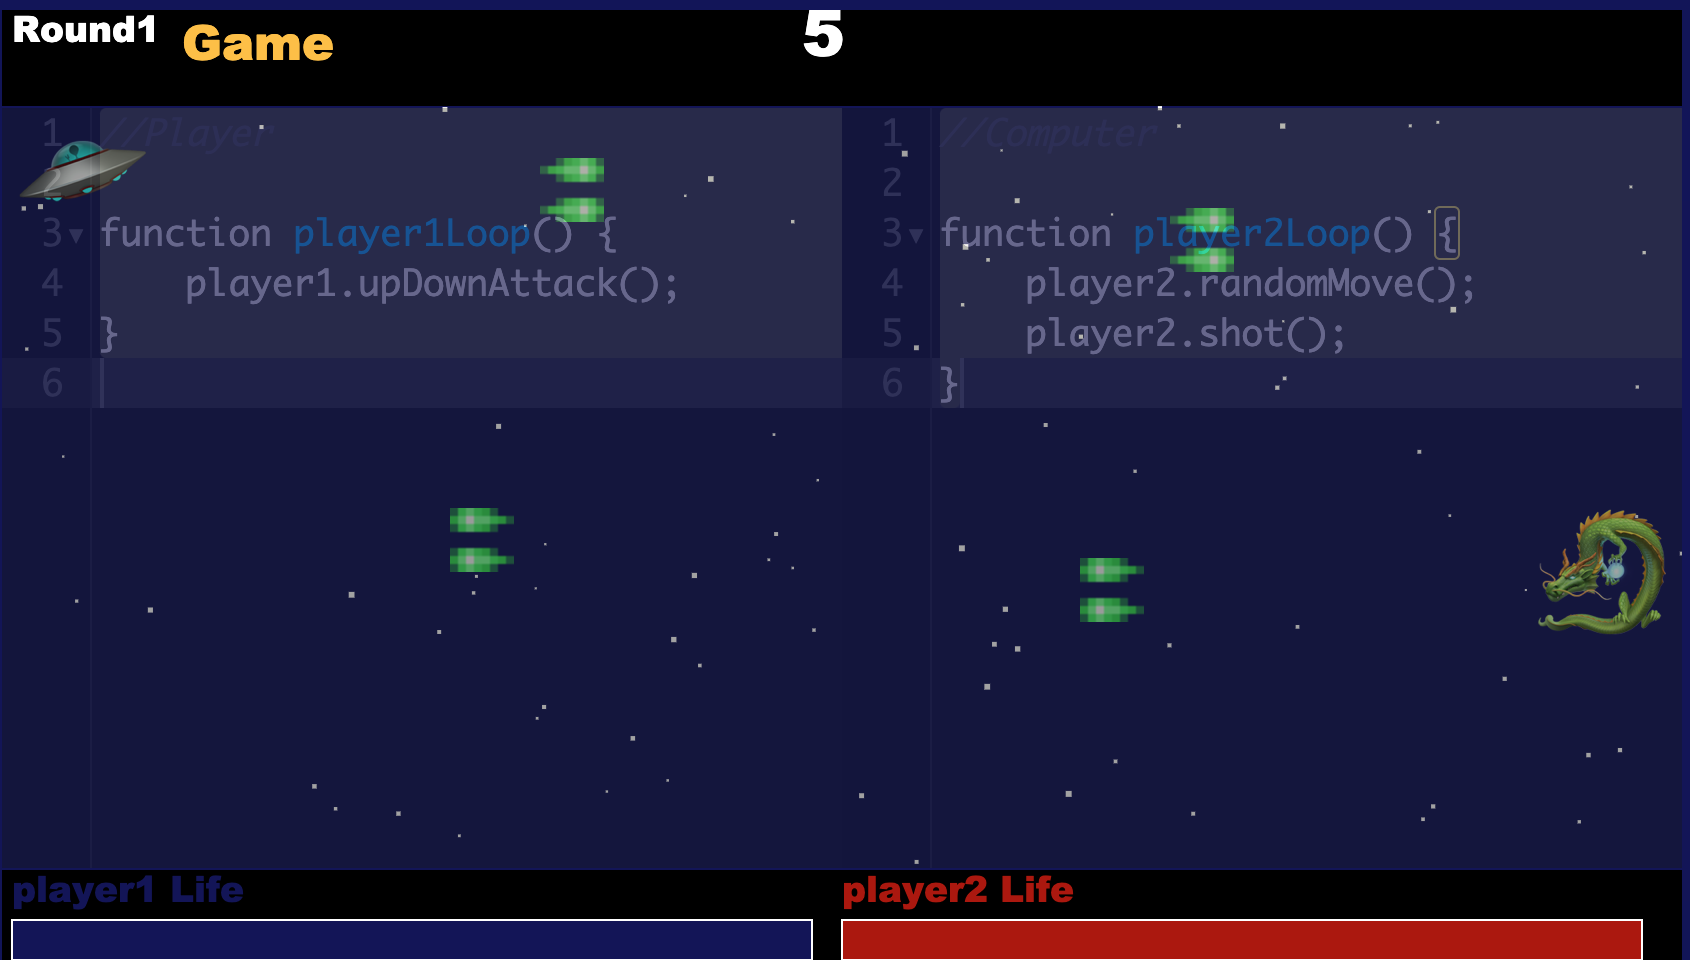
\includegraphics[width=1.0\linewidth]{image/game.eps}
  \end{center}
    \vspace{-8mm} 
  \caption{ゲームフェイズの様子}
  \label{game}
\end{figure}

\subsection{評価実験}
提案システムの使用・観戦に関する感想や影響,用法を調査するために評価実験を実施した.システムをプレイするプログラマと観戦するプログラミング初学者を集め,システムでの対戦と観戦を実施し,アンケート調査と実際に対戦で使用されたプログラムのログを分析することでシステムを評価した.

\subsubsection{実験参加者}
実際にゲームをプレイするプログラマとしては,プログラミング(主にオブジェクト指向言語)の経験が3年以上ある大学院生2名(男性)に声をかけた.2名とも日常的にアクションやシューティング等のジャンルのゲームをプレイするため,システムをプレイする際にゲームに不慣れなためハンデが生まれることはないと思われる.また両者とも3年以上JavaScriptを使用した経験がある.
またプレイを観戦するプログラミング初学者は,国際人間科学部にて開講されていた講義「プログラミング基礎演習1」の受講者をとした.受講者のうち,実験に参加した者は77名であり,うち37名が男性,40名が女性であった.またこの講義ではJavaScriptにおける変数,条件分岐,繰り返しなどの基礎的な文法を教えており,実験参加者は実験を行う時点でこれらを学習済であった.なお,うち23名は授業以前にプログラミングを学習した経験があったが,ソフトウェア開発を行ったことのある者はいなかった.
またプログラマ含む実験参加者の全員が,競技プログラミングやプログラミングゲームなどのプログラミングを題材としたエンタテインメントを使用した経験がなかった.

\subsubsection{実験内容}

初めにプログラマ2人に簡単な事前アンケートを行った後,提案システムにある程度慣れ,用法を理解してもらう必要があるため,システムの練習をするための期間を設けた.システムの使用方法,ゲームシステム,独自に用意したメソッドなどについて説明した後,11/13から11/19の1週間システムを自由に使用させた.また,ただシステムを使用させただけではゲームに対する理解度が上がらない可能性があるため,期間中に2つのタスクをこなさせた.1つは1人以上とシステムを使った対人戦を行うことであり,もう1つは相手がランダムな戦略を実行してくる対CPU戦において,勝率が高いと考えられるプログラムを作成することである.なお期間中はシステムに関する意見・疑問を逐次報告させ,システム使用における問題を改善した.
練習期間が終わった翌日に,プログラマ同士の対戦を行った.対戦はシステムに関するプログラマ同士のコミュニケーション等の所作を観察するため,感染症対策を徹底した環境で対面にて行った.両者の対戦時の画面を録画し,対戦後にシステムに関する事後アンケートを行った.なお練習期間中・対戦中にプログラマが記述した全てのコードのログを収集した.
そして「プログラミング基礎演習1」の最終講義で受講者に事前アンケートを行った後,初学者が観戦しやすいように対戦動画を編集したものをzoomを介して閲覧させた.またその後にシステムに関する事後アンケートを行った.

\subsubsection{実験結果}

\begin{enumerate}
  \item アンケート結果

  \begin{table}[h]
    \centering
    \caption{初学者に対する事後アンケート結果}
    \label{beginner_interview}
      \begin{tabular}{|c|c|c|c|c|c|c|c|} \hline
        \multirow{2}{*}{Q} & \multirow{2}{*}{質問項目} & \multicolumn{5}{c}{評価分布} & \multirow{2}{*}{平均} \\
        & & 1 & 2 & 3 & 4 & 5 & \\ \hline\hline
        Q1 & ゲームを観戦するのは楽しかったか & 3 & 6 & 33 & 27 & 5 & 3.34\\ \hline
        Q2 & ゲームの出力はプログラムを理解する助けになったか & 0 & 9 & 25 & 30 & 10 & 3.55\\ \hline
        Q3 & 観戦によってプログラミングに対する興味関心は高まったか & 1 & 11 & 23 & 33 & 6 & 3.43\\ \hline
        Q4 & 観戦によってプログラミングに関する理解が深まったか & 1 & 23 & 29 & 17 & 4 & 3.00\\ \hline
      \end{tabular}
  \end{table}

  対戦を観戦したプログラミング初学者に対する事後アンケートの内容及び結果を表\ref{interview}に示す.まずゲーム観戦の楽しさに関して(Q1)であるが,実験参加者の多くが肯定的な回答を示した.またキャラクタが攻撃,移動するなどのゲームの出力がプログラム理解の助けになったかという質問(Q2)に関しても3以上の評価が多かった.また観戦によりプログラミングに対する興味関心が高まったかという質問(Q3)についても,3以上の回答が多くなった.また観戦によってプログラミングに関する理解が深まったかという質問(Q4)に関しては,やや低い評価が多い結果となった.またこれら意外にも以下の質問をした.

  \begin{itemize}
    \item Q5.このゲームを実際にプレイしたいか(プレイしたい/プレイしたくない)
    \item Q6.このゲームに他にどのような機能が欲しいか
    \item Q7.このゲームに関する意見
  \end{itemize}

  まずこのゲームを実際にプレイしたいかという質問(Q5)に関しては64.9\%がプレイしたいと回答した.またこのゲームに他にどのような機能が欲しいかという質問(Q6)に関しては「色んな技が繰り出せるような機能」「通常攻撃以外にため技のようなものが欲しいと思った」「回復アイテム的なものや必殺技」「攻撃を受けたときの衝撃波」などの回答があり,キャラクタの行動,エフェクト,アイテムの追加などを求める意見が多く見られた.また「プログラム内容を解説する機能が欲しい」という意見も複数あり,Q4の結果にも見られるように,プログラムの内容をより分かりやすくする工夫が必要だと考えられる.またこのゲームに関する意見(Q7)としては,「自分のプログラミングのレベルを上げたいと思った」「面白い」「プログラミングを楽しみながら学習できると言う点でとても面白いと感じた」などゲームに対する肯定的な意見が多く得られた.しかし「プログラミング初心者には少し難しかった」「楽しめるようになるまでのハードルが高そうだった」「今持っている知識では自分では動かすことが出来ないと感じた」などゲームをプレイするのは難しそうだという反応も多く得られた.
  またシステムをプレイしたプログラマにも同様に事後アンケートを行った.その内容・結果を表\ref{interview}に示す.

  \begin{table}[h]
    \centering
    \caption{プログラマに対する事後アンケート結果}
    \label{programmer_interview}
      \begin{tabular}{|c|c|c|c|} \hline
        Q & 質問項目 & プログラマA & プログラマB \\ \hline
        Q1 & システムをプレイするのは楽しかったか & 4 & 5 \\ \hline
        Q2 & ゲームの出力はプログラムを理解する助けになったか & 4 & 5\\ \hline
        Q3 & プレイすることでプログラミングに対する興味関心は高まったか & 3 & 5\\ \hline
        Q4 & プレイによってプログラミングに関する理解が深まったか & 1 & 3\\ \hline
      \end{tabular}
  \end{table}
  この結果についても初学者に対する事後アンケートと同様の傾向があり,Q1,Q2,Q3については肯定的な評価が得られたが,Q4に関してはやや評価が低い結果となった.またそれら以外にも以下の質問をした.

  \begin{itemize}
    \item Q5.累計何時間程度システムを使用したか
    \item Q6.ゲームの難易度は自分にとって適切だったか
    \item Q7.どのような点が簡単(難しい)と感じたか
    \item Q8.ゲームに他にどのような機能が欲しいか
    \item Q9.今後もこのゲームを使用したいか
    \item Q10.ゲームに関する意見
  \end{itemize}

  累計何時間程度システムを使用したかという質問(Q5)に関しては1名が2時間,1名が6時間と回答した.またゲームの難易度は自分にとって適切だったかという質問(Q6)に関しては1名が適切だった,1名がやや難しかったと答えた.具体的には(Q7)「リファレンスが乏しくプログラムを書きづら買った」「現状のシステムではある程度システムを使い込んだ人をを想定した作戦を立てづらかった」と回答した.ゲームに他にどのような機能が欲しいかという質問(Q8)に対しては,「オブジェクトが持っている値を確認できるリファレンスのようなものが欲しい」「横移動ができれば,被弾しやすいリスクと引き換えに,敵が来そうな位置で敵より先に弾を打ち込めるチャンスが増える」と回答していた.また今後もこのゲームを使用したいか(Q9)という質問には2名とも「使用したい」と回答した.なおゲームに関する意見は「相手のコードを読んで対処するという部分をもっと積極的にするべきだったかもしれない.ただし,相手の位置に近づくようにプログラムすれば確実に自分が先に被弾するので,自分は動かずに相手が近づくのを待つプログラム以外最良の手がないようにも思う.」というものが得られた.

  \item コードログ分析結果
  練習期間中・対戦中にプログラマが記述したプログラムのログ,提出したプログラムを分析することで,システムがどのように利用されているか,どのようなプログラムが記述されているかを調査した.
  まずvsComputerモードで使用されたコードの分析結果について述べる.このモードで使用されたコードは合計件である.全てのコードに含まれていたキーワード(演算子を除く)の個数をグラフ化したものを図\ref{vsComputer_keyword}に示す.


  \begin{figure}[!h]
    \begin{center}
      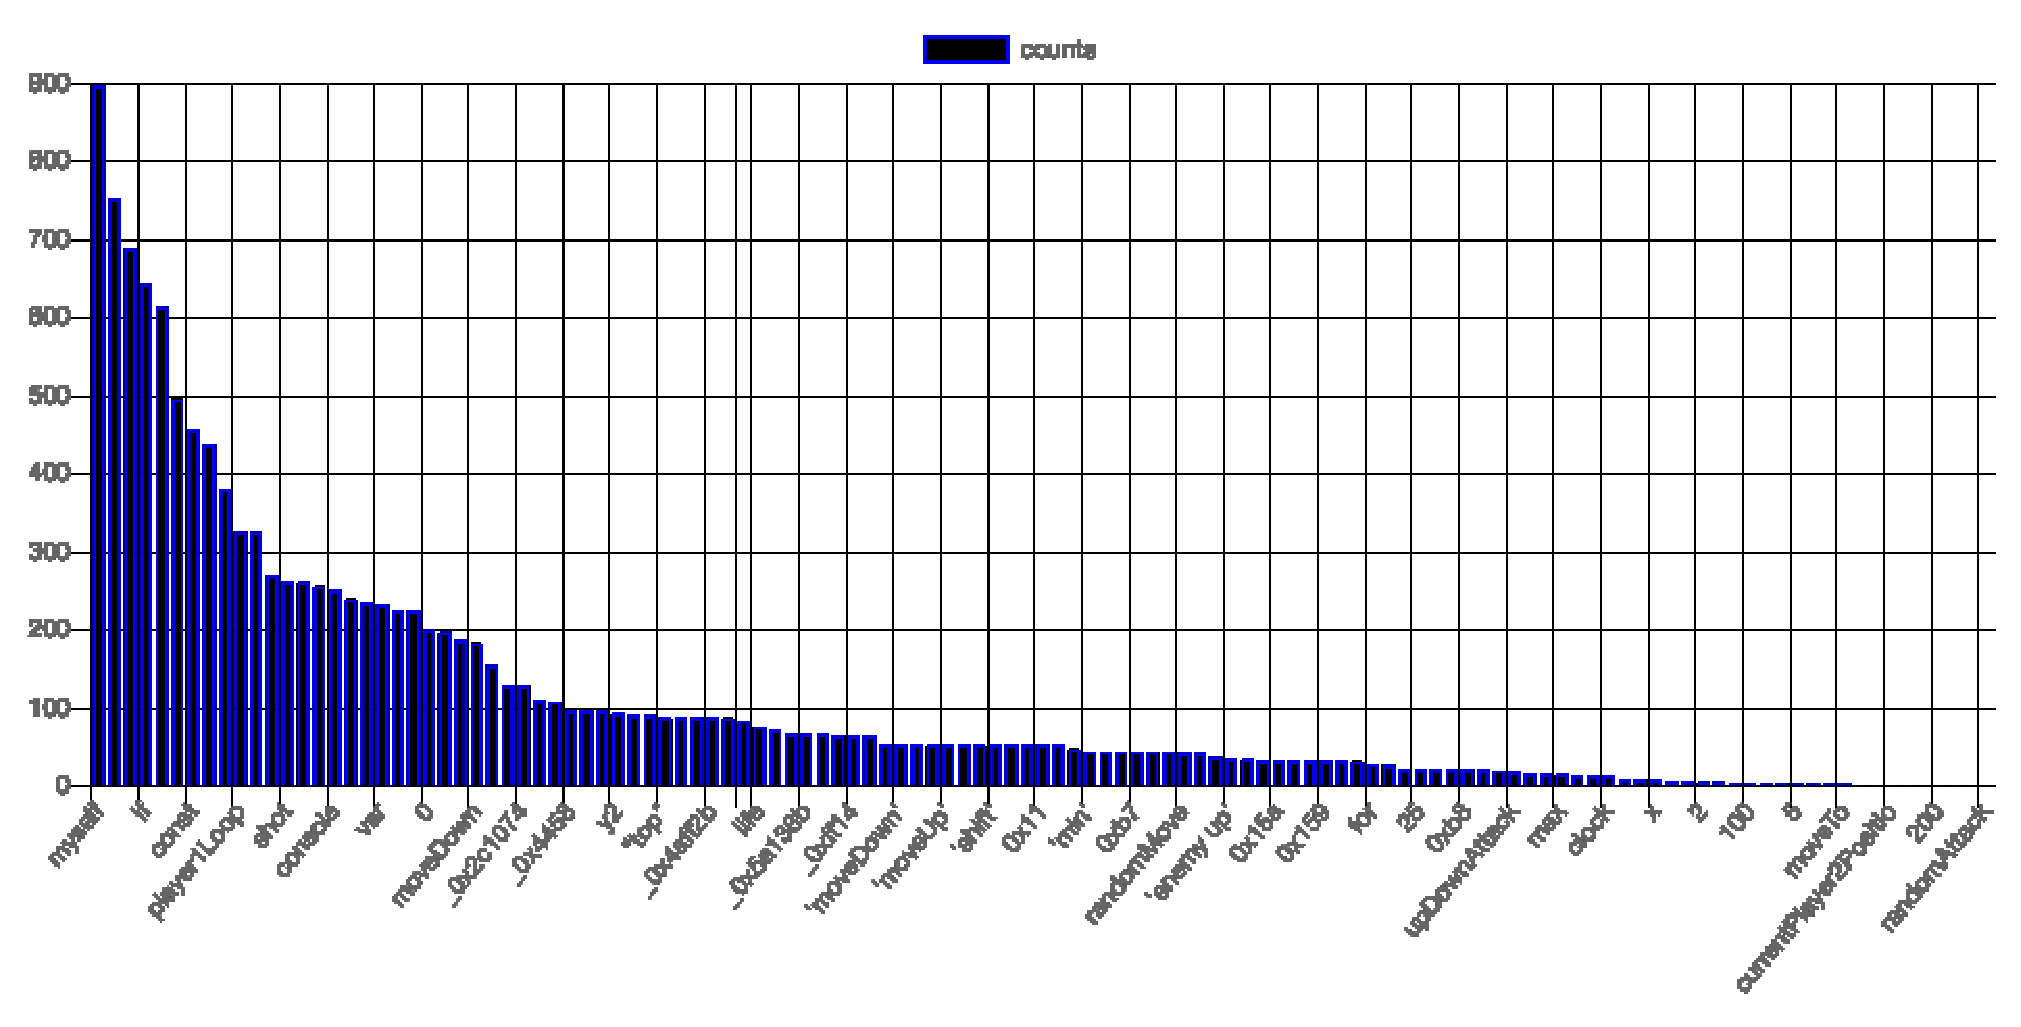
\includegraphics[width=1.0\linewidth]{image/vsComputer_result.eps}
    \end{center}
      \vspace{-8mm} 
    \caption{vsComputerにおけるキーワード分析}
    \label{vsComputer_keyword}
  \end{figure}
\end{enumerate}

\subsubsection{考察}
評価実験に関する考察について述べる.プログラマ同士の対戦においては,行動プログラミングフェイズで設定したappearanceについて「かわいい」などとコメントしていた.また対戦後にお互いのプログラムの内容や今までのプログラミング経験に関するコミュニケーションをとっており,システムを使用することでプログラマ同士のコミュニケーションを促進できていたと考えられる.
初学者の対戦の観戦においては,ライブでプログラマ同士が対戦している状況を用意することが困難であったため今回は動画を閲覧するという状況を用意したが,動画を見ただけでは実際に人が対戦しているという感覚が希薄であり,「プログラマがプログラミングしている」場面を見せるためには更なる工夫が必要であると感じた.
また今回の評価実験において,システムに対する肯定的な評価が得られたものの,どのような要素が初学者のプログラミングに対する興味に影響を与えていたのか,特に提案システムにおいて独特な要素であるリアルタイムな駆け引き・アドリブを誘発する要素の影響について調査する必要があると考えられる.

\subsection{課題}



\newpage
\section{まとめ}

% 本論文では,プロジェクションマッピングによる情報提示を行うウェアラブルデバイスにより,紙の書籍による読書体験を拡張するシステムを提案した.提案システムはウェブカメラから取得した紙面の画像を取得し,光学文字認識により紙面の文章データを得る.そして取得した文章を形態素解析により形態素に分け,名詞のみを抽出し,紙面に表示する.ユーザが紙面に表示された名詞を選択すると,その名詞の意味または関連画像が検索され,紙面上に表示される.このシステムを用いて読書することにより,読者は分からない名詞が出てきた際にも,読書を中断して辞書や電子書籍で調べることなく調べ物が可能で,より拡張された読書を体験できると考えられる.
% 提案システムが,実際に読書の利便性を高められているか,実装した機能について調査した.その結果,デバイスの機能に関しては便利だという意見が得られたが,文字・画像の表示位置,トラッキングの精度と入力インタフェースに改善すべき点が見つかった.
% 今後の課題として,トラッキング精度を改善し,より適切な位置へ情報を投影することが必要である.入力インタフェースとして用いたLeapMotionが使いづらいという意見が多く寄せられたため,読書行為を阻害しないインタフェースの検討が必要である.なおデバイスの情報処理に時間がかかり,文字・画像の投影タイミングが遅いという結果も得られたため,プログラム内容の簡略化やより高速な言語を使用してのシステム開発が必要だと考えられる.


\newpage
\addcontentsline{toc}{section}{\protect\numberline{}{謝辞}}
\markright{}
\section*{謝辞}

本研究を行うにあたり,日頃より御指導,御激励を賜り,数々の御教示を頂きまし
た西田健志准教授に深甚なる謝恩の意を表します.また神戸大学大学院国際文化学研究科に在学中,御教示,御激励頂いた神戸大学大学院国際文化学研究科の諸先生方に感謝すると共に,諸職員の方々に感謝いたします.日頃より数々の御助言を下さいました諸先輩方,快適な環境を作って頂いた研究室の皆様方,実験に協力頂いた実験参加者の方々に深く感謝いたします.特に研究活動に対する多くのアドバイスとサポートを頂いた工学研究科の清水友順氏,国際文化学研究科の三嶋哲也氏に深く感謝いたします.

\newpage
\addcontentsline{toc}{section}{\protect\numberline{}{参考文献}}
\markright{}
\begin{thebibliography}{99}
	
	%はじめに
	\bibitem{survey}諸外国におけるプログラミング教育に関する調査研究, \url{https://www.mext.go.jp/a_menu/shotou/zyouhou/detail/__icsFiles/afieldfile/2018/08/10/programming_syogaikoku_houkokusyo.pdf}.
	\bibitem{guide}小学校プログラミング教育の手引(第三版), \url{https://www.mext.go.jp/content/20200218-mxt_jogai02-100003171_002.pdf}.
	\bibitem{matsumoto}松本 絵里子, 佐藤良樹, 佐藤瑞帆ほか: C言語の概念と実行過程を可視化するプログラミング学習用アプリケーションの開発,専修ネットワーク&インフォメーション, No.24, pp.15-26 (2016).
	
	%コードリーディング関連
	\bibitem{progate}Progate, \url{https://prog-8.com/}.
	\bibitem{gist}GitHub Gist, \url{https://gist.github.com/}.

	\bibitem{mitani}三谷将大, 寺田実: Webアプリケーションによるゲーミフィケーションを用いたプログラミング上達支援システム, 第27 回インタラクティブシステムとソフトウェアに関するワークショップ, (Sept.2018).

	\bibitem{guzman}E.Guzman et al: Sentiment analysis of commit comments in GitHub: an empirical study, In Proceedings of the 11th Working Conference on Mining Software Repositories, 2014, pp. 352--355.
	\bibitem{nagano}永野真知, 早瀬康裕, 駒水孝裕, 北川博之: GitHubとStackOverflowにおけるユーザ行動の統一的な分析, 情報処理学会第79回全国大会, pp. 363–364 (Mar. 2017).
	\bibitem{shibatou}柴藤大介, 有薗拓也, 宮崎章太, 矢谷浩司: CodeGlass:GitHubのプルリクエストを活用したコード断片のインタラクティブな調査支援システム, 情報処理学会インタラクション, vol.2019, pp.159–16 (Mar. 2019).
	\bibitem{ichinose}一ノ瀬智浩, 畑秀明, 松本健一: ソースコード上の技術的負債除去を活性化させるゲーミフィケーション環境の開発, 情報処理学会関西支部支部大会講演論文集, vol.2016, (Sept. 2016).
	\bibitem{hikawa}樋川一幸, 松田滉平, 中村聡史: コミュニケーションチャネルに入り込む研究室実験BOTの提案と運用, 情報処理学会研究報告グループウェアとネットワークサービス,vol.3, pp. 1–7(Mar. 2019).
	\bibitem{omura}大村裕, 渡部卓雄: プログラム理解のためのコードリーディング支援ツールの提案と実装, 日本ソフトウェア科学会講演論文集, vol.31, pp.443–446, (Sep. 2014).
	\bibitem{ishio}石尾隆, 田中昌弘, 井上克郎: ソースコード上での情報タグ伝播によるコードリーディング支援, ウィンターワークショップ論文集, Vol.2008, pp.31–32, (Jan. 2008).

	\bibitem{uww2019}Ubiquitous Wearable Workshop, \url{http://cse.eedept.kobe-u.ac.jp/uww2019/}.

	%プログラミングゲーム関連

	%プログラミングを用いたエンタテインメント
	\bibitem{topcoder}Topcoder, \url{https://www.topcoder.com/}.
	\bibitem{codegolf}浜地慎一郎: Code Golf, \url{http://shinh.skr.jp/dat_dir/golf_prosym.pdf}.
	\bibitem{seccon}SECCON, \url{https://www.seccon.jp}.
	\bibitem{robocode}Robocode, \url{https://robocode.sourceforge.io/}.

	%プログラミング教育システム
	\bibitem{tsukamoto}T. Hidekuni, et al.: Textual vs. visual programming languages in programming education for primary schoolchildren, 2016 IEEE Frontiers in Education Conference (FIE), IEEE, 2016. p.. 1--7.
	\bibitem{scratch}Scratch, \url{https://scratch.mit.edu/}.
	\bibitem{viscuit}Viscuit, \url{https://www.viscuit.com/}.
	\bibitem{dolittle}S.Kanemune et al: Dolittle: an object-oriented language for K12 education, EuroLogo, 2005, pp. 144--153.

	%ライブコーディング環境
	\bibitem{livecodelab}LivecodeLab, \url{https://livecodelab.net/}.
	\bibitem{hydra}Hydra, \url{https://hydra.ojack.xyz/}.

	%プログラミングゲームを使った研究
	\bibitem{long}L.Ju: Just For Fun: using programming games in software programming training and education, Journal of Information Technology Education: Research, 2007, pp. 279--290.
	\bibitem{joshua}J.Shi et al: Pyrus: Designing A Collaborative Programming Game to Promote Problem Solving Behaviors, Proceedings of the 2019 CHI Conference on Human Factors in Computing Systems, No. 656, pp. 1–12 (May.2019).
	\bibitem{minakuchi}水口充: 成績評価のためのプログラミングゲームの設計と実践, 研究報告エンタテインメントコンピューティング(EC), vol. 2016, pp. 1–7(July.2016).

	\bibitem{mashitani}増谷海人, 赤澤紀子: 仮想現実を用いた初学者向けプログラミング学習システムの提案, 2018年度情報処理学会関西支部支部大会講演論文集,vol. 2018, (Sept.2018).

	\bibitem{esprima}Esprima, \url{https://esprima.org/}.
	\bibitem{escomplex}escomplex, \url{https://github.com/escomplex/escomplex}.

\end{thebibliography}


\end{document}